\subsection*{4.1 Herzscher Dipol}
    Elektrisches Pendel: Kondensator und Spule sind Energiespeicher.
    Wenn das magnetische Feld abgebaut wird, so wird das elektrische aufgebaut und umgekehrt.
    Idealisiert (ohne Reibung) "pendelt" dieses System unendlich lange
    \centering
    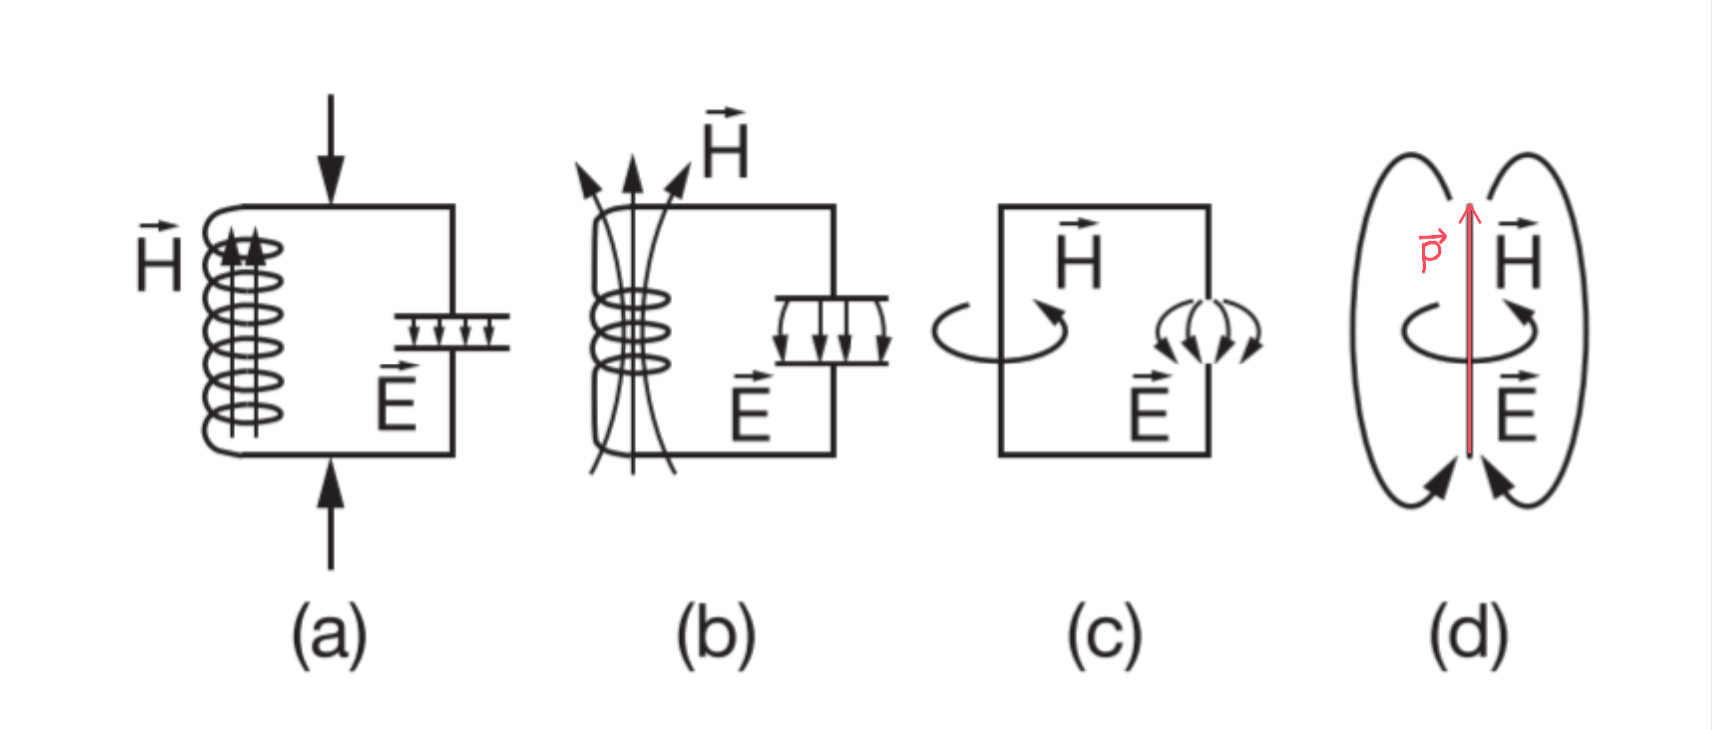
\includegraphics[height = 30mm]{src/images/herzscher_dipol.png}

    Dipolmoment $\overrightarrow{p}$ (alternierende Richtung durch Wechselspannung):
    \mathbox{\overrightarrow{p} = q \overrightarrow{l} = \overrightarrow{p_0} cos(\omega t)}

    Fernfeld: Entfernt man sich weit vom Sender (Herzschen Dipol), so verschwindet der phasenunterschied zwischen elektrischem und magnetischem Feld.

    \mathbox{\overrightarrow{E} = \overrightarrow{E_0} cos(\omega t - k r)}
    \mathbox{\overrightarrow{H} = \overrightarrow{H_0} cos(\omega t - k r)}
    mit Kreisfrequenz $\omega = 2 \pi \nu \rightarrow T = \frac{1}{\nu}$, Wellenzahl $k = \frac{2 \pi}{\lambda}$
    [$\nu = $ Frequenz, $T = $ Periode, $\lambda = $ Wellenlänge]